\documentclass[svgnames,smaller]{beamer}\usepackage[]{graphicx}\usepackage[]{color}
% maxwidth is the original width if it is less than linewidth
% otherwise use linewidth (to make sure the graphics do not exceed the margin)
\makeatletter
\def\maxwidth{ %
  \ifdim\Gin@nat@width>\linewidth
    \linewidth
  \else
    \Gin@nat@width
  \fi
}
\makeatother

\definecolor{fgcolor}{rgb}{0.345, 0.345, 0.345}
\newcommand{\hlnum}[1]{\textcolor[rgb]{0.686,0.059,0.569}{#1}}%
\newcommand{\hlstr}[1]{\textcolor[rgb]{0.192,0.494,0.8}{#1}}%
\newcommand{\hlcom}[1]{\textcolor[rgb]{0.678,0.584,0.686}{\textit{#1}}}%
\newcommand{\hlopt}[1]{\textcolor[rgb]{0,0,0}{#1}}%
\newcommand{\hlstd}[1]{\textcolor[rgb]{0.345,0.345,0.345}{#1}}%
\newcommand{\hlkwa}[1]{\textcolor[rgb]{0.161,0.373,0.58}{\textbf{#1}}}%
\newcommand{\hlkwb}[1]{\textcolor[rgb]{0.69,0.353,0.396}{#1}}%
\newcommand{\hlkwc}[1]{\textcolor[rgb]{0.333,0.667,0.333}{#1}}%
\newcommand{\hlkwd}[1]{\textcolor[rgb]{0.737,0.353,0.396}{\textbf{#1}}}%
\let\hlipl\hlkwb

\usepackage{framed}
\makeatletter
\newenvironment{kframe}{%
 \def\at@end@of@kframe{}%
 \ifinner\ifhmode%
  \def\at@end@of@kframe{\end{minipage}}%
  \begin{minipage}{\columnwidth}%
 \fi\fi%
 \def\FrameCommand##1{\hskip\@totalleftmargin \hskip-\fboxsep
 \colorbox{shadecolor}{##1}\hskip-\fboxsep
     % There is no \\@totalrightmargin, so:
     \hskip-\linewidth \hskip-\@totalleftmargin \hskip\columnwidth}%
 \MakeFramed {\advance\hsize-\width
   \@totalleftmargin\z@ \linewidth\hsize
   \@setminipage}}%
 {\par\unskip\endMakeFramed%
 \at@end@of@kframe}
\makeatother

\definecolor{shadecolor}{rgb}{.97, .97, .97}
\definecolor{messagecolor}{rgb}{0, 0, 0}
\definecolor{warningcolor}{rgb}{1, 0, 1}
\definecolor{errorcolor}{rgb}{1, 0, 0}
\newenvironment{knitrout}{}{} % an empty environment to be redefined in TeX

\usepackage{alltt}
\usetheme[progressbar=none, numbering=fraction]{metropolis}

% define colors
\setbeamercolor{frametitle}{bg=SteelBlue}
\setbeamercolor{progress bar}{fg=SteelBlue}
\setbeamercolor{background canvas}{bg=White}

\newcounter{saveenumerate}
\makeatletter
\newcommand{\enumeratext}[1]{%
\setcounter{saveenumerate}{\value{enum\romannumeral\the\@enumdepth}}
\end{enumerate}
#1
\begin{enumerate}
\setcounter{enum\romannumeral\the\@enumdepth}{\value{saveenumerate}}%
}
\makeatother

\setlength{\leftmargini}{2em}

% \setbeamertemplate{itemize items}[default]
% \setbeamertemplate{enumerate items}[default]

\usepackage{amsmath}
\usepackage{amsfonts}
\usepackage{bm}
\usepackage{hyperref}
\hypersetup{
    colorlinks=true,
    linkcolor=magenta,
    filecolor=magenta,      
    urlcolor=magenta,
}
\setbeamertemplate{footline}{}
\setbeamertemplate{logo}{%
    \usebeamercolor[fg]{footline}%
    \usebeamerfont{page number in head/foot}%
  \usebeamertemplate*{frame numbering}\hspace{6pt}%
}

\usepackage{booktabs}
\usepackage{multirow}
\usepackage{pgf, tikz}
\usepackage{tkz-tab}
\usetikzlibrary{shapes,decorations,arrows,calc,arrows.meta,fit,positioning}
\usetikzlibrary{arrows,shapes.arrows,shapes.geometric,shapes.multipart,
decorations.pathmorphing,positioning}
\tikzstyle{arrow}=[->, >=stealth]
\tikzset{
    -Latex,auto,node distance =1 cm and 1 cm,semithick,
    state/.style ={ellipse, draw, minimum width = 0.7 cm},
    cond/.style ={rectangle, draw, minimum width = 0.7 cm},
    point/.style = {circle, draw, inner sep=0.04cm,fill,node contents={}},
    bidirected/.style={Latex-Latex,dashed},
    el/.style = {inner sep=2pt, align=left, sloped}
}
\usepackage{subcaption}
\usepackage{caption}

\usepackage{tcolorbox}
\tcbuselibrary{listings,breakable, skins}
\newcommand\dummy[1]{#1}
\let\Begin\begin
\let\End\end
\newenvironment{tcbmagenta}[1]
    {\dummy{\Begin{tcolorbox}[enhanced, breakable=true, title = #1, colback=white, colframe=magenta!75]}
    }
    {
    \End{tcolorbox}
    }


\usepackage{dirtree}

% magenta bold command
\newcommand{\bmagenta}[1]{\textcolor{magenta}{\textbf{#1}}}

% mathhbb E
\newcommand{\E}{\mathbb{E}}

\newcommand{\indep}{\perp \!\!\! \perp}
\IfFileExists{upquote.sty}{\usepackage{upquote}}{}
\begin{document}




%%%%%%%%%%%%%%%%%%%%
%% TITLE FRAME
%%%%%%%%%%%%%%%%%%%%%%%%%%%%%%%%%%%%%%%%%%%%%%%%%%%%%%%%%%%%%%%%%%%%%%%%%%%%%%%%%%%%%% TITLE
{
\setbeamercolor{background canvas}{bg=SteelBlue!30}
\begin{frame}
\begin{center}
\vspace{0cm}\large \textcolor{SteelBlue!95}{\textbf{Getting started with R}} \\

{\color{Snow}\hrulefill}

\textcolor{SteelBlue!95}{Matt Lee (mlee8@g.harvard.edu), PHS Launch 2022}
\end{center}
\end{frame}
}

\small

%%%%%%%%%%%%%%%%%%%%%%%%%%%%%%%%%%%%%%%%%%%%%%%%%%%%%%%%%%
%%
%%  What is R
%%
%%%%%%%%%%%%%%%%%%%%%%%%%%%%%%%%%%%%%%%%%%%%%%%%%%%%%%%%%%

\begin{frame}{What is R?}

\begin{itemize}
    \item R is an open-source \textbf{interpreted} programming language: when you install R, you install an \textit{interpreter} that translates your R code into computer code (sometimes called ``machine'' code), which is what actually gets run
    \item This is in contrast to \textbf{compiled} languages (e.g. C or C++), where the programmer writes code that is directly converted into machine code
    \item Several advantages of interpreted languages: much more user friendly, easily read, consistent across operating systems
    \item Some disadvantages: often slower, and less control over system hardware$^*$
\end{itemize}

\vspace{1em}

\bmagenta{Action step:} Install R (https://cloud.r-project.org/) 

\end{frame}


%%%%%%%%%%%%%%%%%%%%%%%%%%%%%%%%%%%%%%%%%%%%%%%%%%%%%%%%%%
%%
%%  R studio
%%
%%%%%%%%%%%%%%%%%%%%%%%%%%%%%%%%%%%%%%%%%%%%%%%%%%%%%%%%%%

\begin{frame}{R Studio: Integrated Development Environments (IDEs)}

\begin{itemize}
    \item We can interact with R directly via a command line (e.g. Terminal)
    \begin{figure}[tb]
    \centering
    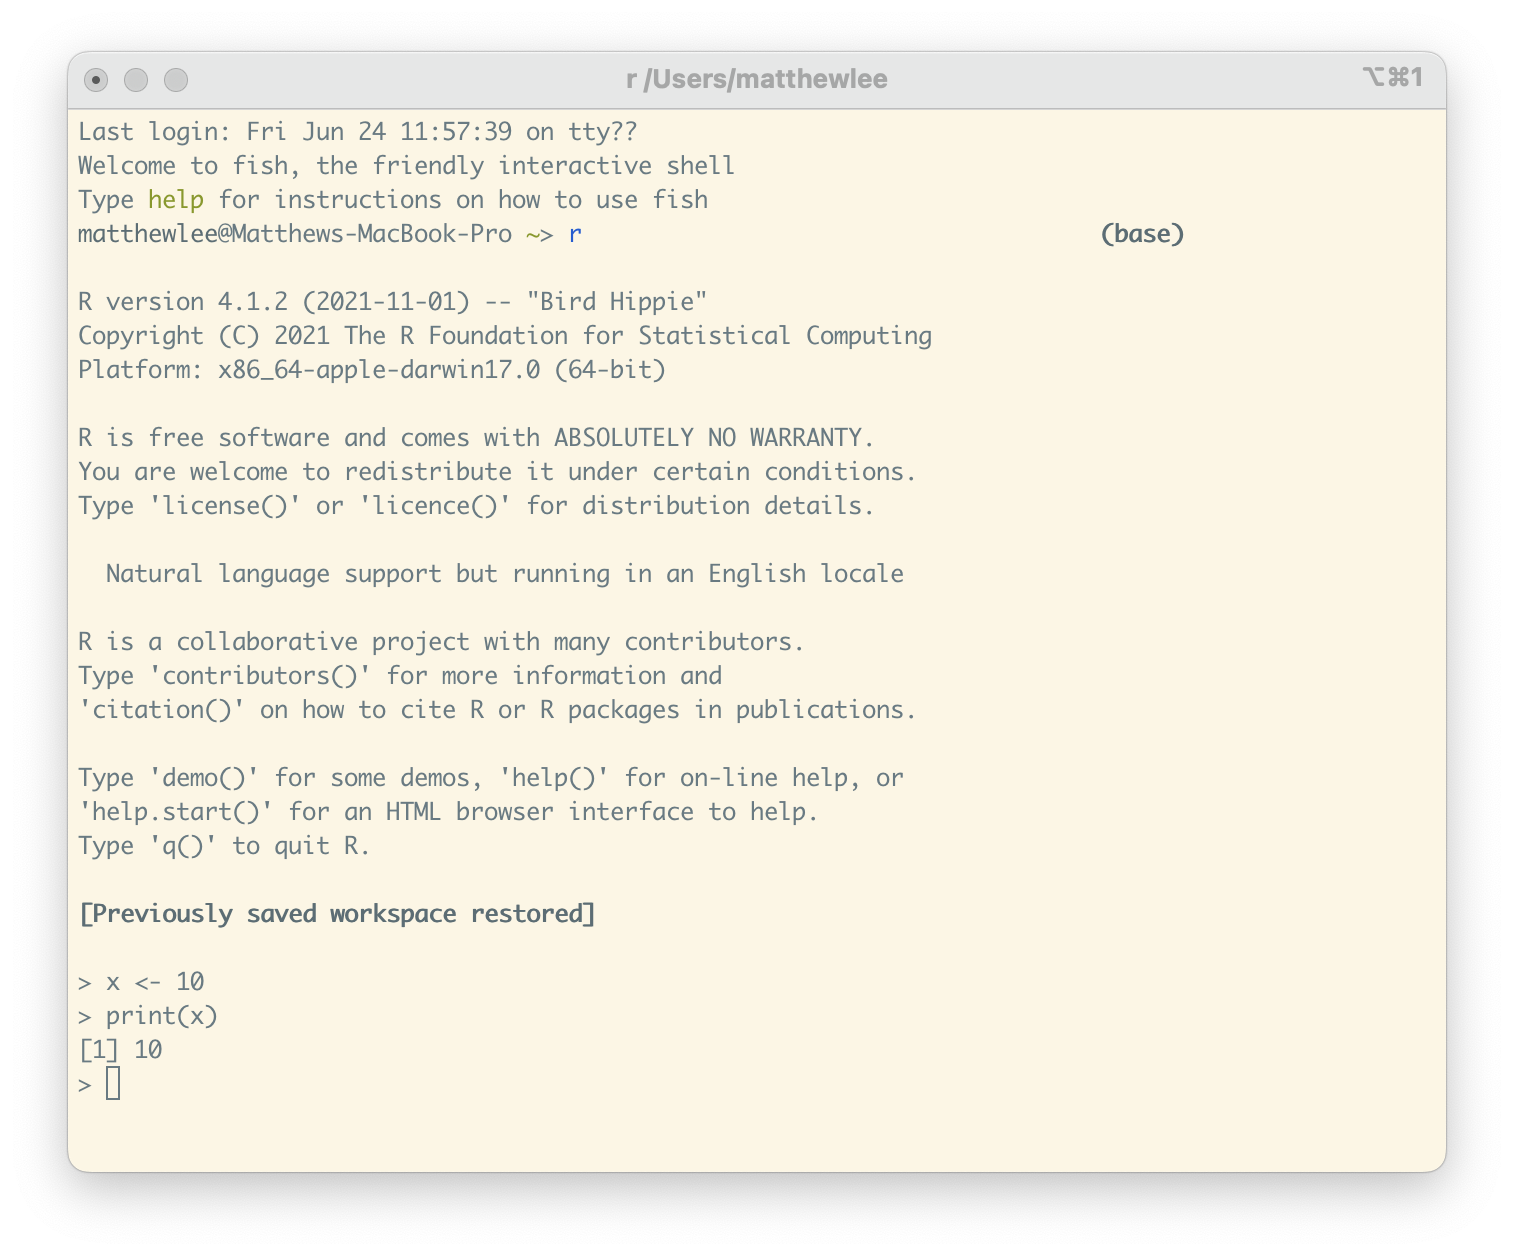
\includegraphics[width = .35\textwidth]{R-terminal.png}
    \end{figure}
    \item But this is not very pretty or reproducible! A population alternative is to use an IDE, such as R Studio, which is a program that adds a whole lot of convenience to writing and running R code
    \item IDEs are not the language themselves, they provide a way to interact with the language installed on your computer in a friendly way
\end{itemize}

\bmagenta{Action step:} Install R Studio (https://www.rstudio.com/products/rstudio/download/) 


\end{frame}


%%%%%%%%%%%%%%%%%%%%%%%%%%%%%%%%%%%%%%%%%%%%%%%%%%%%%%%%%%
%%
%%  Working in R Studio
%%
%%%%%%%%%%%%%%%%%%%%%%%%%%%%%%%%%%%%%%%%%%%%%%%%%%%%%%%%%%

\begin{frame}{Working in R Studio}

Key R Studio panes:
\begin{itemize}
    \item Console: Runs R code, either interactively or via an R script
    \item Terminal: Convenient terminal application (primarily useful for version control programs like git/GitHub)
    \item Environment: Objects you've saved to your \textbf{working R environment}
    \item Files: File navigator, useful if you need to figure out where data/R scripts are located
    \item Plots: Plots generated will populate in this pane -- you can also export plots you create using the ``Export'' button
\end{itemize}

\end{frame}


%%%%%%%%%%%%%%%%%%%%%%%%%%%%%%%%%%%%%%%%%%%%%%%%%%%%%%%%%%
%%
%%  R scripts
%%
%%%%%%%%%%%%%%%%%%%%%%%%%%%%%%%%%%%%%%%%%%%%%%%%%%%%%%%%%%

\begin{frame}{R Scripting}

Use of an \textbf{R script} helps keep your code neat and reproducible
\begin{itemize}
    \item In R Studio: File $\rightarrow$ New File $\rightarrow$ R Script
    \item This is simply a text file with the extension ``.R'' that will hold all of the R commands we want to run
    \item Similar to other languages, ``\#'' is reserved for comments
\end{itemize}

There are 5 main \textbf{data types} in R:
\begin{itemize}
    \item Character (e.g. \texttt{"hello world"})
    \item Numeric (e.g. \texttt{3.14159265})
    \item Integer (e.g. \texttt{5L})
    \item Logical (\texttt{TRUE}, \texttt{FALSE})
    \item Complex (\texttt{1i})
\end{itemize}

Other special values include missing (\texttt{NA}), not-a-number (\texttt{NaN}), null (\texttt{NULL}), and infinity (\texttt{Inf}, \texttt{-Inf})

\end{frame}

%%%%%%%%%%%%%%%%%%%%%%%%%%%%%%%%%%%%%%%%%%%%%%%%%%%%%%%%%%
%%
%%  R scripts
%%
%%%%%%%%%%%%%%%%%%%%%%%%%%%%%%%%%%%%%%%%%%%%%%%%%%%%%%%%%%

\begin{frame}[fragile]{R Scripting}

R also has various \textbf{data structures}, but the main ones are:
\begin{itemize}
    \item Vectors: a collection of elements of one data type
    \item Lists: a collection of objects of arbitrary types (e.g. the first element could be a vector, the second element could be a matrix, the third element could be a data frame)
    \item Matrices: a vector with dimensions defined
    \item Data frames: structure that most resembles a data set, each variable is a single data type
    \item Factors: a numeric vector that has a label attribute (like a Stata label)
\end{itemize}


R is also built on \textbf{functions}, some of which are provided in the base installation and others that can be installed or created from scratch:

\begin{knitrout}\scriptsize
\definecolor{shadecolor}{rgb}{0.969, 0.969, 0.969}\color{fgcolor}\begin{kframe}
\begin{alltt}
\hlkwd{a_function_with_3_args}\hlstd{(}\hlkwc{arg1} \hlstd{= ...,} \hlkwc{arg2} \hlstd{= ...,} \hlkwc{arg3} \hlstd{= ...)}
\end{alltt}
\end{kframe}
\end{knitrout}
Functions take \textbf{arguments} or inputs, and return \textbf{values} (in R parlance) or outputs. 

\end{frame}


%%%%%%%%%%%%%%%%%%%%%%%%%%%%%%%%%%%%%%%%%%%%%%%%%%%%%%%%%%
%%
%%  R Basics
%%
%%%%%%%%%%%%%%%%%%%%%%%%%%%%%%%%%%%%%%%%%%%%%%%%%%%%%%%%%%

\begin{frame}[fragile]{R Basics}

Creating a vector, then assigning it to the variable \texttt{x} or \texttt{y}:

\begin{knitrout}\scriptsize
\definecolor{shadecolor}{rgb}{0.969, 0.969, 0.969}\color{fgcolor}\begin{kframe}
\begin{alltt}
\hlcom{# "<-" is the assignment operator}
\hlstd{x} \hlkwb{<-} \hlkwd{c}\hlstd{(}\hlnum{1}\hlstd{,} \hlnum{2}\hlstd{,} \hlnum{3}\hlstd{)} \hlcom{# c() is a function! }
\hlkwd{print}\hlstd{(x)}
\end{alltt}
\begin{verbatim}
## [1] 1 2 3
\end{verbatim}
\begin{alltt}
\hlcom{# short hand for sequences of numbers}
\hlstd{y} \hlkwb{<-} \hlnum{1}\hlopt{:}\hlnum{3}
\hlkwd{print}\hlstd{(y)}
\end{alltt}
\begin{verbatim}
## [1] 1 2 3
\end{verbatim}
\begin{alltt}
\hlcom{# vectors can contain strings}
\hlstd{a_string} \hlkwb{<-} \hlkwd{c}\hlstd{(}\hlstr{"hello"}\hlstd{,} \hlstr{"world"}\hlstd{)}
\hlkwd{print}\hlstd{(a_string)}
\end{alltt}
\begin{verbatim}
## [1] "hello" "world"
\end{verbatim}
\end{kframe}
\end{knitrout}

\end{frame}

%%%%%%%%%%%%%%%%%%%%%%%%%%%%%%%%%%%%%%%%%%%%%%%%%%%%%%%%%%
%%
%%  R Basics
%%
%%%%%%%%%%%%%%%%%%%%%%%%%%%%%%%%%%%%%%%%%%%%%%%%%%%%%%%%%%

\begin{frame}[fragile]{R Basics}

What type of vector is \texttt{what\_type}:

\begin{knitrout}\scriptsize
\definecolor{shadecolor}{rgb}{0.969, 0.969, 0.969}\color{fgcolor}\begin{kframe}
\begin{alltt}
\hlstd{what_type} \hlkwb{<-} \hlkwd{c}\hlstd{(}\hlnum{1}\hlstd{,} \hlstr{"hello"}\hlstd{)}
\hlkwd{print}\hlstd{(what_type)}
\end{alltt}
\begin{verbatim}
## [1] "1"     "hello"
\end{verbatim}
\end{kframe}
\end{knitrout}

\end{frame}

%%%%%%%%%%%%%%%%%%%%%%%%%%%%%%%%%%%%%%%%%%%%%%%%%%%%%%%%%%
%%
%%  R Basics
%%
%%%%%%%%%%%%%%%%%%%%%%%%%%%%%%%%%%%%%%%%%%%%%%%%%%%%%%%%%%

\begin{frame}[fragile]{R Basics}

Generating matrices and data frames:

\begin{knitrout}\scriptsize
\definecolor{shadecolor}{rgb}{0.969, 0.969, 0.969}\color{fgcolor}\begin{kframe}
\begin{alltt}
\hlstd{my_mat} \hlkwb{<-} \hlkwd{matrix}\hlstd{(}\hlkwc{data} \hlstd{=} \hlkwd{c}\hlstd{(}\hlnum{1}\hlopt{:}\hlnum{9}\hlstd{),} \hlkwc{nrow} \hlstd{=} \hlnum{3}\hlstd{,} \hlkwc{ncol} \hlstd{=} \hlnum{3}\hlstd{)}
\hlkwd{print}\hlstd{(my_mat)}
\end{alltt}
\begin{verbatim}
##      [,1] [,2] [,3]
## [1,]    1    4    7
## [2,]    2    5    8
## [3,]    3    6    9
\end{verbatim}
\begin{alltt}
\hlcom{# turning this into a data frame}
\hlstd{my_df} \hlkwb{<-} \hlkwd{data.frame}\hlstd{(my_mat)}
\hlkwd{print}\hlstd{(my_df)}
\end{alltt}
\begin{verbatim}
##   X1 X2 X3
## 1  1  4  7
## 2  2  5  8
## 3  3  6  9
\end{verbatim}
\end{kframe}
\end{knitrout}

\end{frame}


%%%%%%%%%%%%%%%%%%%%%%%%%%%%%%%%%%%%%%%%%%%%%%%%%%%%%%%%%%
%%
%%  R Basics
%%
%%%%%%%%%%%%%%%%%%%%%%%%%%%%%%%%%%%%%%%%%%%%%%%%%%%%%%%%%%

\begin{frame}[fragile]{R Basics}

Indexing into 2-dimensional matrices and data frames:

\begin{knitrout}\scriptsize
\definecolor{shadecolor}{rgb}{0.969, 0.969, 0.969}\color{fgcolor}\begin{kframe}
\begin{alltt}
\hlstd{my_mat} \hlkwb{<-} \hlkwd{matrix}\hlstd{(}\hlkwc{data} \hlstd{=} \hlkwd{c}\hlstd{(}\hlnum{1}\hlopt{:}\hlnum{9}\hlstd{),} \hlkwc{nrow} \hlstd{=} \hlnum{3}\hlstd{,} \hlkwc{ncol} \hlstd{=} \hlnum{3}\hlstd{)}
\hlkwd{print}\hlstd{(my_mat[}\hlnum{2}\hlstd{,}\hlnum{3}\hlstd{])} \hlcom{# bracket method [row, column]}
\end{alltt}
\begin{verbatim}
## [1] 8
\end{verbatim}
\begin{alltt}
\hlstd{my_df} \hlkwb{<-} \hlkwd{data.frame}\hlstd{(my_mat)}
\hlkwd{print}\hlstd{(my_df}\hlopt{$}\hlstd{X1)}  \hlcom{# pulling out a column of a data.frame}
\end{alltt}
\begin{verbatim}
## [1] 1 2 3
\end{verbatim}
\begin{alltt}
\hlkwd{print}\hlstd{(my_df[,}\hlnum{1}\hlstd{])} \hlcom{# brackets work here too}
\end{alltt}
\begin{verbatim}
## [1] 1 2 3
\end{verbatim}
\begin{alltt}
\hlkwd{print}\hlstd{(my_df[}\hlnum{2}\hlstd{,}\hlnum{3}\hlstd{])}
\end{alltt}
\begin{verbatim}
## [1] 8
\end{verbatim}
\end{kframe}
\end{knitrout}

\end{frame}


%%%%%%%%%%%%%%%%%%%%%%%%%%%%%%%%%%%%%%%%%%%%%%%%%%%%%%%%%%
%%
%%  R Basics
%%
%%%%%%%%%%%%%%%%%%%%%%%%%%%%%%%%%%%%%%%%%%%%%%%%%%%%%%%%%%

\begin{frame}[fragile]{R Basics}

R does math (e.g. \texttt{+, -,  *, /, >, >=, ==}):

\begin{knitrout}\scriptsize
\definecolor{shadecolor}{rgb}{0.969, 0.969, 0.969}\color{fgcolor}\begin{kframe}
\begin{alltt}
\hlcom{# rnorm() simulates draws from normal distributions}
\hlstd{x} \hlkwb{<-} \hlkwd{rnorm}\hlstd{(}\hlkwc{n} \hlstd{=} \hlnum{10}\hlstd{,} \hlkwc{mean} \hlstd{=} \hlnum{0}\hlstd{,} \hlkwc{sd} \hlstd{=} \hlnum{3}\hlstd{)}
\hlkwd{print}\hlstd{(x)}
\end{alltt}
\begin{verbatim}
##  [1] -5.7411212 -0.8227805  3.6030561  2.5185614  5.1350010 -4.7169971
##  [7]  2.8750995  0.3494500  3.2149292  4.7576505
\end{verbatim}
\begin{alltt}
\hlkwd{head}\hlstd{(x)} \hlcom{# what does head do? }
\end{alltt}
\begin{verbatim}
## [1] -5.7411212 -0.8227805  3.6030561  2.5185614  5.1350010 -4.7169971
\end{verbatim}
\begin{alltt}
\hlkwd{mean}\hlstd{(x)}
\end{alltt}
\begin{verbatim}
## [1] 1.117285
\end{verbatim}
\begin{alltt}
\hlstd{x[}\hlnum{1}\hlstd{]} \hlopt{+} \hlstd{x[}\hlnum{2}\hlstd{]} \hlcom{# indexing for vectors (i.e. a 1-dimension matrix)}
\end{alltt}
\begin{verbatim}
## [1] -6.563902
\end{verbatim}
\end{kframe}
\end{knitrout}

\end{frame}


%%%%%%%%%%%%%%%%%%%%%%%%%%%%%%%%%%%%%%%%%%%%%%%%%%%%%%%%%%
%%
%%  R Basics
%%
%%%%%%%%%%%%%%%%%%%%%%%%%%%%%%%%%%%%%%%%%%%%%%%%%%%%%%%%%%

\begin{frame}[fragile]{R Basics}

Many of these operators can also be used to index in more nuanced ways: 
\begin{knitrout}\scriptsize
\definecolor{shadecolor}{rgb}{0.969, 0.969, 0.969}\color{fgcolor}\begin{kframe}
\begin{alltt}
\hlstd{x} \hlkwb{<-} \hlkwd{c}\hlstd{(}\hlnum{1}\hlstd{,} \hlnum{2}\hlstd{,} \hlnum{3}\hlstd{,} \hlnum{4}\hlstd{,} \hlnum{5}\hlstd{,} \hlnum{5}\hlstd{)}

\hlcom{# indexing using operators}
\hlstd{x} \hlopt{<} \hlnum{3}
\end{alltt}
\begin{verbatim}
## [1]  TRUE  TRUE FALSE FALSE FALSE FALSE
\end{verbatim}
\begin{alltt}
\hlstd{x[x} \hlopt{<} \hlnum{3}\hlstd{]}
\end{alltt}
\begin{verbatim}
## [1] 1 2
\end{verbatim}
\begin{alltt}
\hlstd{x[x} \hlopt{==} \hlnum{7}\hlstd{]}
\end{alltt}
\begin{verbatim}
## numeric(0)
\end{verbatim}
\begin{alltt}
\hlstd{x[x} \hlopt{==} \hlnum{5}\hlstd{]}
\end{alltt}
\begin{verbatim}
## [1] 5 5
\end{verbatim}
\end{kframe}
\end{knitrout}

\end{frame}


%%%%%%%%%%%%%%%%%%%%%%%%%%%%%%%%%%%%%%%%%%%%%%%%%%%%%%%%%%
%%
%%  R Basics
%%
%%%%%%%%%%%%%%%%%%%%%%%%%%%%%%%%%%%%%%%%%%%%%%%%%%%%%%%%%%

\begin{frame}[fragile]{R Basics}

Beware default behavior for missing data:

\begin{knitrout}\scriptsize
\definecolor{shadecolor}{rgb}{0.969, 0.969, 0.969}\color{fgcolor}\begin{kframe}
\begin{alltt}
\hlstd{x} \hlkwb{<-} \hlkwd{c}\hlstd{(}\hlnum{1}\hlstd{,} \hlnum{3}\hlstd{,} \hlnum{5}\hlstd{,} \hlnum{NA}\hlstd{)}
\hlkwd{print}\hlstd{(x)}
\end{alltt}
\begin{verbatim}
## [1]  1  3  5 NA
\end{verbatim}
\begin{alltt}
\hlkwd{mean}\hlstd{(x)}
\end{alltt}
\begin{verbatim}
## [1] NA
\end{verbatim}
\begin{alltt}
\hlkwd{mean}\hlstd{(x,} \hlkwc{na.rm} \hlstd{=} \hlnum{TRUE}\hlstd{)}
\end{alltt}
\begin{verbatim}
## [1] 3
\end{verbatim}
\end{kframe}
\end{knitrout}

\texttt{na.rm = TRUE} is an example of an \textbf{optional argument} we can pass to the \texttt{mean()} function, telling R to ignore the missing values

\end{frame}


%%%%%%%%%%%%%%%%%%%%%%%%%%%%%%%%%%%%%%%%%%%%%%%%%%%%%%%%%%
%%
%%  R Basics Check
%%
%%%%%%%%%%%%%%%%%%%%%%%%%%%%%%%%%%%%%%%%%%%%%%%%%%%%%%%%%%

\begin{frame}[fragile]{R Basics: Check in}

\bmagenta{Complete the following for understanding.} In an R script:
\begin{enumerate}
    \item Create a vector, \texttt{z} $ = \{0, 0, 4, 6, 7, 10\}$
    \item Print the first 3 elements of \texttt{z}
    \item Calculate the standard deviation of \texttt{z} (\textit{hint: look at the sd() function. Entering ``?sd'' in the R console will bring up its documentation. What arguments does this function take?})
    \item Replace the 4th element of \texttt{z} with \texttt{NaN} (\textit{hint: combine what you know about indexing with the assignment operator})
    \item Calculate the standard deviation of this new vector
    \item Save the R script with this code to your desktop folder
\end{enumerate}


\end{frame}


%%%%%%%%%%%%%%%%%%%%%%%%%%%%%%%%%%%%%%%%%%%%%%%%%%%%%%%%%%
%%
%%  R Basics for data
%%
%%%%%%%%%%%%%%%%%%%%%%%%%%%%%%%%%%%%%%%%%%%%%%%%%%%%%%%%%%

\begin{frame}[fragile]{R Basics for Data}

A general pipeline for working with data (in R or any other language) is to: 
\begin{enumerate}
    \item Read in the raw data
    \item Clean data (saved to a new object)
    \item Analyze data
    \item Produce results
\end{enumerate}


\end{frame}

%%%%%%%%%%%%%%%%%%%%%%%%%%%%%%%%%%%%%%%%%%%%%%%%%%%%%%%%%%
%%
%%  R Basics for data
%%
%%%%%%%%%%%%%%%%%%%%%%%%%%%%%%%%%%%%%%%%%%%%%%%%%%%%%%%%%%

\begin{frame}[fragile]{R Basics for Data}

Data can be read into R in various ways depending on the type of file -- the base installation includes functions to read in CSV files:
\begin{knitrout}\scriptsize
\definecolor{shadecolor}{rgb}{0.969, 0.969, 0.969}\color{fgcolor}\begin{kframe}
\begin{alltt}
\hlstd{my_data} \hlkwb{<-} \hlkwd{read.csv}\hlstd{(}\hlstr{"path/to/csv_file.csv"}\hlstd{)}
\end{alltt}
\end{kframe}
\end{knitrout}

For other types of data files, other packages may need to be installed:
\begin{knitrout}\scriptsize
\definecolor{shadecolor}{rgb}{0.969, 0.969, 0.969}\color{fgcolor}\begin{kframe}
\begin{alltt}
\hlkwd{install.packages}\hlstd{(}\hlstr{"haven"}\hlstd{)}
\hlkwd{library}\hlstd{(haven)}
\hlstd{my_stata_data} \hlkwb{<-} \hlkwd{read_dta}\hlstd{(}\hlstr{"path/to/stata_file.dta"}\hlstd{)}

\hlkwd{install.packages}\hlstd{(}\hlstr{"openxlsx"}\hlstd{)}
\hlkwd{library}\hlstd{(openxlsx)}
\hlstd{my_xlsx_data} \hlkwb{<-} \hlkwd{read.xlsx}\hlstd{(}\hlstr{"path/to_excel_file.xlsx"}\hlstd{)}
\end{alltt}
\end{kframe}
\end{knitrout}


\end{frame}


%%%%%%%%%%%%%%%%%%%%%%%%%%%%%%%%%%%%%%%%%%%%%%%%%%%%%%%%%%
%%
%%  R Basics for data
%%
%%%%%%%%%%%%%%%%%%%%%%%%%%%%%%%%%%%%%%%%%%%%%%%%%%%%%%%%%%

\begin{frame}[fragile]{R Basics for Data}

For example, let's say we have a file called "dat.csv" that's located in my desktop folder, with variables for age and whether an individual is an Aquarius:


\begin{knitrout}\scriptsize
\definecolor{shadecolor}{rgb}{0.969, 0.969, 0.969}\color{fgcolor}\begin{kframe}
\begin{alltt}
\hlstd{my_data} \hlkwb{<-} \hlkwd{read.csv}\hlstd{(}\hlstr{"/Users/matthewlee/Desktop/dat.csv"}\hlstd{)}
\end{alltt}
\end{kframe}
\end{knitrout}

Basic summary of the data:
\begin{knitrout}\scriptsize
\definecolor{shadecolor}{rgb}{0.969, 0.969, 0.969}\color{fgcolor}\begin{kframe}
\begin{alltt}
\hlkwd{summary}\hlstd{(my_data)}
\end{alltt}
\begin{verbatim}
##       age           aquarius     
##  Min.   :18.00   Min.   :0.0000  
##  1st Qu.:27.00   1st Qu.:0.0000  
##  Median :29.00   Median :0.0000  
##  Mean   :29.49   Mean   :0.4998  
##  3rd Qu.:32.00   3rd Qu.:1.0000  
##  Max.   :41.00   Max.   :1.0000
\end{verbatim}
\begin{alltt}
\hlkwd{nrow}\hlstd{(my_data)}
\end{alltt}
\begin{verbatim}
## [1] 5000
\end{verbatim}
\end{kframe}
\end{knitrout}


\end{frame}



%%%%%%%%%%%%%%%%%%%%%%%%%%%%%%%%%%%%%%%%%%%%%%%%%%%%%%%%%%
%%
%%  R Basics for data
%%
%%%%%%%%%%%%%%%%%%%%%%%%%%%%%%%%%%%%%%%%%%%%%%%%%%%%%%%%%%

\begin{frame}[fragile]{R Basics for Data}

Let's say we want to generate a new variable, \texttt{notAquarius}, the reciprocal of \texttt{aquarius}. Good practice is to \textbf{not alter the raw data}, so we'll create a copy. In base R we could do:
\begin{knitrout}\scriptsize
\definecolor{shadecolor}{rgb}{0.969, 0.969, 0.969}\color{fgcolor}\begin{kframe}
\begin{alltt}
\hlstd{clean_data} \hlkwb{<-} \hlstd{my_data}

\hlcom{# dollar sign to index the new and old vars}
\hlstd{clean_data}\hlopt{$}\hlstd{notAquarius} \hlkwb{<-} \hlkwd{abs}\hlstd{(}\hlnum{1} \hlopt{-} \hlstd{clean_data}\hlopt{$}\hlstd{aquarius)}
\hlkwd{head}\hlstd{(clean_data)}
\end{alltt}
\begin{verbatim}
##   age aquarius notAquarius
## 1  28        0           1
## 2  30        1           0
## 3  27        1           0
## 4  34        0           1
## 5  30        0           1
## 6  27        0           1
\end{verbatim}
\end{kframe}
\end{knitrout}

\end{frame}

%%%%%%%%%%%%%%%%%%%%%%%%%%%%%%%%%%%%%%%%%%%%%%%%%%%%%%%%%%
%%
%%  R Basics for data
%%
%%%%%%%%%%%%%%%%%%%%%%%%%%%%%%%%%%%%%%%%%%%%%%%%%%%%%%%%%%

\begin{frame}[fragile]{R Basics for Data}

The tidyverse collection of packages, including \texttt{dplyr}, provides some convenient methods for working with data beyond base R. Packages must be installed using the \texttt{install.packages()} function, and loaded using the \texttt{library()} function.

\begin{knitrout}\scriptsize
\definecolor{shadecolor}{rgb}{0.969, 0.969, 0.969}\color{fgcolor}\begin{kframe}
\begin{alltt}
\hlkwd{install.packages}\hlstd{(}\hlstr{"dplyr"}\hlstd{)}
\hlkwd{library}\hlstd{(dplyr)}
\end{alltt}
\end{kframe}
\end{knitrout}

A key feature of \texttt{dplyr} is the \textbf{pipe operator}, denoted by \texttt{\%>\%}, which allows us to feed the results of one function directly into another without creating a new intermediate object.
\begin{knitrout}\scriptsize
\definecolor{shadecolor}{rgb}{0.969, 0.969, 0.969}\color{fgcolor}\begin{kframe}
\begin{alltt}
\hlstd{a_data_frame} \hlopt
    \hlkwd{filter}\hlstd{(x1} \hlopt{>} \hlnum{5}\hlstd{)} \hlopt \hlcom{# filtering to obs where x1 > 5}
    \hlkwd{summarize}\hlstd{(}\hlkwc{mean_of_y} \hlstd{=} \hlkwd{mean}\hlstd{(y))} \hlcom{# mean of y in this subset}
\end{alltt}
\end{kframe}
\end{knitrout}
There is detailed documentation for the many functions in the tidyverse packages, which can be found here at: https://www.tidyverse.org/


\end{frame}

%%%%%%%%%%%%%%%%%%%%%%%%%%%%%%%%%%%%%%%%%%%%%%%%%%%%%%%%%%
%%
%%  R Basics for data
%%
%%%%%%%%%%%%%%%%%%%%%%%%%%%%%%%%%%%%%%%%%%%%%%%%%%%%%%%%%%

\begin{frame}[fragile]{R Basics for Data}

We can use \texttt{dplyr} functions to generate our \texttt{notAquarius} as well using the \texttt{mutate()} function:
\begin{knitrout}\scriptsize
\definecolor{shadecolor}{rgb}{0.969, 0.969, 0.969}\color{fgcolor}\begin{kframe}
\begin{alltt}
\hlstd{clean_data} \hlkwb{<-}
    \hlstd{my_data} \hlopt
    \hlkwd{mutate}\hlstd{(}\hlkwc{notAquarius} \hlstd{=} \hlkwd{abs}\hlstd{(}\hlnum{1} \hlopt{-} \hlstd{aquarius))}
\hlkwd{head}\hlstd{(clean_data)}
\end{alltt}
\begin{verbatim}
##   age aquarius notAquarius
## 1  28        0           1
## 2  30        1           0
## 3  27        1           0
## 4  34        0           1
## 5  30        0           1
## 6  27        0           1
\end{verbatim}
\end{kframe}
\end{knitrout}

\end{frame}

%%%%%%%%%%%%%%%%%%%%%%%%%%%%%%%%%%%%%%%%%%%%%%%%%%%%%%%%%%
%%
%%  R Basics for data
%%
%%%%%%%%%%%%%%%%%%%%%%%%%%%%%%%%%%%%%%%%%%%%%%%%%%%%%%%%%%

\begin{frame}[fragile]{R Basics for Data}

Finally, let's do a basic analysis to compute the proportion of individuals who are an Aquarius by age. Again, \texttt{dplyr} functions make this so simple! 
\begin{knitrout}\scriptsize
\definecolor{shadecolor}{rgb}{0.969, 0.969, 0.969}\color{fgcolor}\begin{kframe}
\begin{alltt}
\hlstd{aqua_age} \hlkwb{<-}
    \hlstd{clean_data} \hlopt
    \hlkwd{group_by}\hlstd{(age)} \hlopt \hlcom{# group by each unique age }
    \hlkwd{summarize}\hlstd{(}\hlkwc{prop_aquarius} \hlstd{=} \hlkwd{mean}\hlstd{(aquarius))}

\hlkwd{nrow}\hlstd{(aqua_age);} \hlkwd{head}\hlstd{(aqua_age)}
\end{alltt}
\begin{verbatim}
## [1] 24
## # A tibble: 6 x 2
##     age prop_aquarius
##   <dbl>         <dbl>
## 1    18         0    
## 2    19         0    
## 3    20         0.857
## 4    21         0.333
## 5    22         0.425
## 6    23         0.568
\end{verbatim}
\end{kframe}
\end{knitrout}
There are quite a few rows to this output, so maybe a table isn't the best way to visualize
\end{frame}

%%%%%%%%%%%%%%%%%%%%%%%%%%%%%%%%%%%%%%%%%%%%%%%%%%%%%%%%%%
%%
%%  R Basics for data
%%
%%%%%%%%%%%%%%%%%%%%%%%%%%%%%%%%%%%%%%%%%%%%%%%%%%%%%%%%%%

\begin{frame}[fragile]{R Basics for Data}

Luckily, R has some great plotting functions:
\begin{knitrout}\scriptsize
\definecolor{shadecolor}{rgb}{0.969, 0.969, 0.969}\color{fgcolor}\begin{kframe}
\begin{alltt}
\hlkwd{plot}\hlstd{(}\hlkwc{x} \hlstd{= aqua_age}\hlopt{$}\hlstd{age,} \hlkwc{y} \hlstd{= aqua_age}\hlopt{$}\hlstd{prop_aquarius,}
     \hlkwc{xlab} \hlstd{=} \hlstr{"Age"}\hlstd{,} \hlkwc{ylab} \hlstd{=} \hlstr{"Propotion Aquarius"}\hlstd{,} \hlkwc{main} \hlstd{=} \hlstr{"Aquarius Plot"}\hlstd{)}
\end{alltt}
\end{kframe}
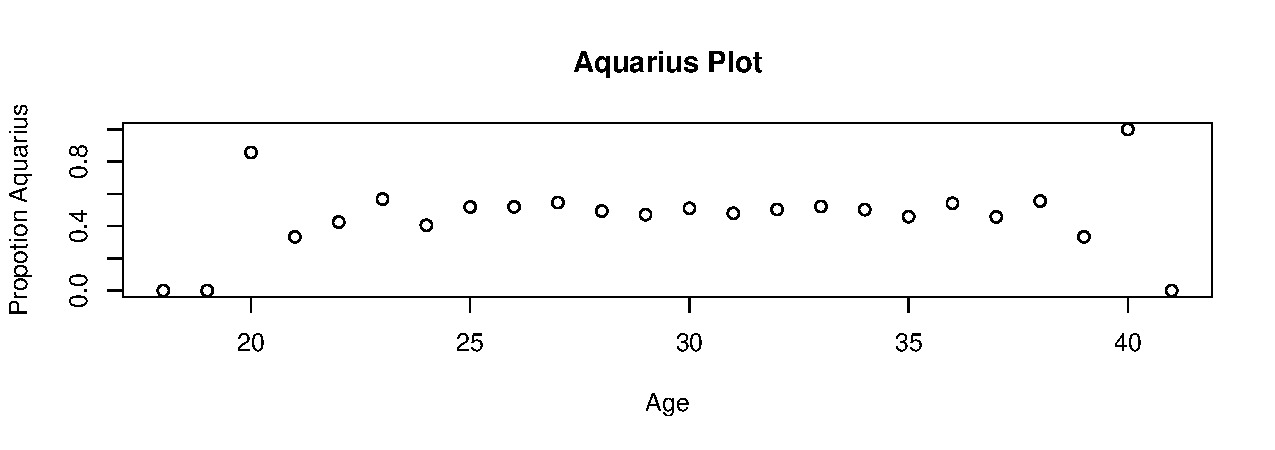
\includegraphics[width=\maxwidth]{figure/unnamed-chunk-20-1} 
\end{knitrout}
\end{frame}


%%%%%%%%%%%%%%%%%%%%%%%%%%%%%%%%%%%%%%%%%%%%%%%%%%%%%%%%%%
%%
%%  R Basics for data
%%
%%%%%%%%%%%%%%%%%%%%%%%%%%%%%%%%%%%%%%%%%%%%%%%%%%%%%%%%%%

\begin{frame}[fragile]{R Basics for Data}

Another popular package for plotting is \texttt{ggplot2}:
\begin{knitrout}\scriptsize
\definecolor{shadecolor}{rgb}{0.969, 0.969, 0.969}\color{fgcolor}\begin{kframe}
\begin{alltt}
\hlkwd{library}\hlstd{(ggplot2)}
\hlkwd{ggplot}\hlstd{(}\hlkwc{data} \hlstd{= aqua_age,}
       \hlkwc{mapping} \hlstd{=} \hlkwd{aes}\hlstd{(}\hlkwc{x} \hlstd{= age,} \hlkwc{y} \hlstd{= prop_aquarius))} \hlopt{+}
    \hlkwd{geom_point}\hlstd{()} \hlopt{+}
    \hlkwd{geom_line}\hlstd{()} \hlopt{+}
    \hlkwd{theme_bw}\hlstd{()} \hlopt{+}
    \hlkwd{labs}\hlstd{(}\hlkwc{title} \hlstd{=} \hlstr{"Aquarius Plot"}\hlstd{,} \hlkwc{x} \hlstd{=} \hlstr{"Age"}\hlstd{,} \hlkwc{y} \hlstd{=} \hlstr{"Proportion Aquarius"}\hlstd{)}
\end{alltt}
\end{kframe}
\end{knitrout}
Elements of ggplots are strung together using the $+$ operator
\begin{itemize}
    \item Plots start with the \texttt{ggplot()} function, which define the data to be plotted as well as the \textit{aesthetics} (e.g. x/y variables, colors, fills, groups)
    \item \texttt{geom\_point()} creates a scatter plot 
    \item \texttt{geom\_line()} then layers on a line plot
    \item \texttt{theme\_bw()} adjusts the basic look of the plot
    \item \texttt{labs()} allows us to assign labels
\end{itemize}

\end{frame}



%%%%%%%%%%%%%%%%%%%%%%%%%%%%%%%%%%%%%%%%%%%%%%%%%%%%%%%%%%
%%
%%  R Basics for data
%%
%%%%%%%%%%%%%%%%%%%%%%%%%%%%%%%%%%%%%%%%%%%%%%%%%%%%%%%%%%

\begin{frame}[fragile]{R Basics for Data}

\begin{knitrout}\scriptsize
\definecolor{shadecolor}{rgb}{0.969, 0.969, 0.969}\color{fgcolor}
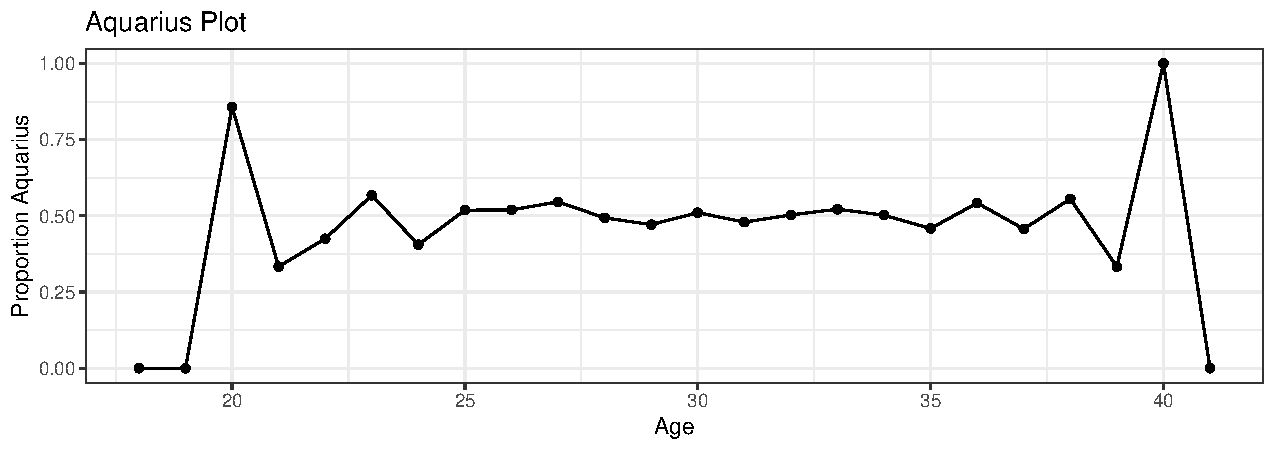
\includegraphics[width=\maxwidth]{figure/unnamed-chunk-22-1} 
\end{knitrout}

\texttt{ggplot2} is another package that has a bunch of functions to customize your plots. Documentation can be found \href{https://ggplot2.tidyverse.org/index.html}{here}
\end{frame}


%%%%%%%%%%%%%%%%%%%%%%%%%%%%%%%%%%%%%%%%%%%%%%%%%%%%%%%%%%
%%
%%  R Data Check
%%
%%%%%%%%%%%%%%%%%%%%%%%%%%%%%%%%%%%%%%%%%%%%%%%%%%%%%%%%%%

\begin{frame}[fragile]{R Basics for Data: Check in}

\bmagenta{Complete the following for understanding.} 
\begin{enumerate}
    \item Download the demographics data from the 2017-18 cycle of NHANES, located \href{https://wwwn.cdc.gov/nchs/nhanes/search/datapage.aspx?Component=Demographics&CycleBeginYear=2017}{here}.
    \item In an R script:
    \begin{enumerate}
        \item Read in this data set (an .xpt file -- you will need a function from the \textbf{haven} package, look up the documentation or Google to figure out which one)
        \item Pick two variables (one continuous, one categorical) of interest using the documentation \href{https://wwwn.cdc.gov/Nchs/Nhanes/2017-2018/DEMO_J.htm}{posted online}, and create a new version of the dataset that only contains these two variables (\textit{hint: the \texttt{select()} function from the dplyr package might be useful})
        \item For the categorical variable, the actual values are probably numeric. Using the NHANES documentation, create a new \textbf{factor} variable that adds informative labels to the original. (\textit{hint: the \texttt{factor()} function might be useful})
        \item Calculate the mean of the continuous variable by levels of the categorical level, and create a plot to show your results.
    \end{enumerate}
\end{enumerate}


\end{frame}


%%%%%%%%%%%%%%%%%%%%%%%%%%%%%%%%%%%%%%%%%%%%%%%%%%%%%%%%%%
%%
%%  R Data Management
%%
%%%%%%%%%%%%%%%%%%%%%%%%%%%%%%%%%%%%%%%%%%%%%%%%%%%%%%%%%%

\begin{frame}{Analysis Management Tips}

Here is a basic organization scheme that I use (prob overkill for classwork):
\dirtree{%
.1 Project folder.
.2 Folder for R code.
.3 R.
.4 readclean.R.
.4 models.R.
.4 create\_tables.R.
.4 create\_figures.R.
.2 out.
.2 run\_analysis.R.
}
\begin{itemize}
    \item The R/ subfolder has general functions I write to clean the data, run the models, and generate results
    \item The out/ folder is where I save all of my output
    \item The run\_analysis.R file is a wrapper script that calls all the functions needed to run through an analysis from start to finish. I usually run this file using the R command \texttt{rmarkdown::render(``run\_analysis.R'')}, which will execute all the commands and generate a nice output file
\end{itemize}
\end{frame}


%%%%%%%%%%%%%%%%%%%%%%%%%%%%%%%%%%%%%%%%%%%%%%%%%%%%%%%%%%
%%
%%  R Tips
%%
%%%%%%%%%%%%%%%%%%%%%%%%%%%%%%%%%%%%%%%%%%%%%%%%%%%%%%%%%%

\begin{frame}{Other R Tips}

\begin{itemize}
    \item If you are unsure what a function does or what arguments it takes, calling ``\texttt{?mean}'' or ``\texttt{??mean}'' will bring up or search help/documentation files
    \item Stack Overflow and Google are your best friends. If you have a question or see an error message, it's likely that someone else has also had the same issue and posted it to an online forum. Copy/pasting your error messages into Google is a good place to start when troubleshooting
    \item R is \textbf{case sensitive}, so a variable called \texttt{newvar} is different than a variable called \texttt{NewVar}
    \item Avoid using R function names for objects, e.g. don't do the following:
\begin{knitrout}\scriptsize
\definecolor{shadecolor}{rgb}{0.969, 0.969, 0.969}\color{fgcolor}\begin{kframe}
\begin{alltt}
\hlstd{mean} \hlkwb{<-} \hlnum{9}
\end{alltt}
\end{kframe}
\end{knitrout}
    \item Sometimes restarting R (or your computer) resolves some issues
    \item R cheat sheets are nice references: https://rstudio.com/resources/cheatsheets/
\end{itemize}
\end{frame}


%%%%%%%%%%%%%%%%%%%%%%%%%%%%%%%%%%%%%%%%%%%%%%%%%%%%%%%%%%
%%
%%  Open questions/work
%%
%%%%%%%%%%%%%%%%%%%%%%%%%%%%%%%%%%%%%%%%%%%%%%%%%%%%%%%%%%

\begin{frame}{Troubleshooting/Q\&A}



\end{frame}





\end{document}
